\documentclass{article}
\usepackage{cite}
\usepackage{listings}
\usepackage{amsmath}
% \usepackage{minted1}
\usepackage{hyperref}
\usepackage{amsfonts}
\usepackage{multicol} \usepackage{fancyheadings} \usepackage{pdfpages}
\usepackage{nips15submit_e,times}
\setlength{\emergencystretch}{10em}

\newtheorem{theorem}{Theorem}[section]
\newtheorem{lemma}[theorem]{Lemma}
\newtheorem{proposition}[theorem]{Proposition}
\newtheorem{corollary}[theorem]{Corollary}
 
\newenvironment{proof}[1][Proof]{\begin{trivlist}
\item[\hskip \labelsep {\bfseries #1}]}{\end{trivlist}}
\newenvironment{definition}[1][Definition]{\begin{trivlist}
\item[\hskip \labelsep {\bfseries #1}]}{\end{trivlist}}
\newenvironment{example}[1][Example]{\begin{trivlist}
\item[\hskip \labelsep {\bfseries #1}]}{\end{trivlist}}
\newenvironment{remark}[1][Remark]{\begin{trivlist}
\item[\hskip \labelsep {\bfseries #1}]}{\end{trivlist}}

\DeclareMathOperator*{\Exp}{\mathbb{E}}
\DeclareMathOperator*{\Prob}{\mathbf{P}}


\lstdefinelanguage{JavaScript}{
      morekeywords={break, case, catch, continue, debugger, default, delete,         do, else, false, finally, for, function, if, in, instanceof, new, null, return, switch, this, throw, true, try, typeof, var, void, while, with},
      morecomment=[s]{/*}{*/},
      morecomment=[l]//,
      morestring=[b]",
      morestring=[b]'
    }
  \lstset{language=JavaScript, xleftmargin=0.5in}

\title{Qualitative Probabilistic Programming}


\author{
Jessica Taylor \\
Department of Computer Science\\
Stanford University \\
Stanford, CA 94305
\texttt{jessica.liu.taylor@gmail.com}
\And
Andreas Stuhlm\"uller \\
Department of Brain and Cognitive Sciences \\
MIT \\
Cambridge, MA 02139 \\
\texttt{andreas@stuhlmueller.org}
\And
Noah Goodman \\
Department of Psychology \\
Stanford University \\
Stanford, CA 94305
\texttt{ngoodman@stanford.edu}
}

\newcommand{\fix}{\marginpar{FIX}}
\newcommand{\new}{\marginpar{NEW}}

%\nipsfinalcopy % Uncomment for camera-ready version

\begin{document}

  \maketitle

  \begin{abstract}
    In probabilistic programs, sometimes it is difficult to specify the correct
    parameterized family of distributions.  We explore an extension to
    probabilistic programming languages that allows programmers to mark some
    distributions as unspecified.  Then, we can fill in the distribution with
    some family and infer parameters.
  \end{abstract}

   % TODO syntax coloring

  \section{Introduction}

  By separating model specification and inference, probabilistic programming 
  has made it easier for non-experts to implement and use probabilistic models.
  Practitioners frequently have strong intuitions about the {\em structure}
  of their domain knowledge, such as which latent variables exist and what
  their causal relations are, and probabilistic programming allows them to encode
  this knowledge. However, it also requires them to specify the specific parametric
  shape and parameterization of any distributions used, and intuitions tend to
  be much less precise there.
  We present Quipp, a system that does {\em not} require such specification;
  instead, random variables and random functions can be left undefined
  and will automatically be filled in under maximum entropy assumptions
  based on their types and available datasets.
  
  Our formalism can concisely express a wide variety of models that machine
  learning practitioners care about, and we provide an expectation
  maximization algorithm that can learn the parameters for many of
  these models with reasonable efficiency. This system makes it easy
  for non-experts to encode their beliefs about the data and to get
  predictions based on as few additional assumptions as possible.
  
  % This feature has multiple advantages.  First, it is easier to write
  % models without knowing about the class of models being used.  This should
  % make probabliistic programming more accessible to non-experts.  Secondly,
  % parameter inference is more efficient if specialized algorithms are used
  % rather than the generic algorithms used to infer other random variables
  % (such as Metropolis Hastings).

  % We define an example probabilistic programming language with this feature
  % (Quipp) and show how it can be used to write machine learning models
  % concisely.

  In an ordinary probabilistic programming language (such as Church),
  it is possible to treat parameters as random variables.  This
  would allow ordinary inference algorithms to infer parameters.  However,
  there are advantages of having unknown functions as a feature
  in the language.
  First, it is easier to
  write programs without knowing the details of different parameterized distributions.
  Second, the system can use specialized algorithms to infer parameters faster.

  % Inference in these models is performed using the expectation-maximization
  % algorithm, with alternating steps of inferring latent variables and optimizing
  % parameters.

  % - Motivation for Quipp
  %   - Explanation of "unknown functions"
  %   - Writing machine learning algorithms as probabilistic programs
  %   - Accessibility to non-experts
  %   - Comparison to existing probabilistic programming languages
  %     - In other languages, use random variables for parameters
  %     - Random variables slower because they are updated independently

  In the following, we first specify the syntax used to write Quipp programs,
  including the notation for unknown variables and functions.
  We describe the class of exponential family variables and functions that our system can learn,
  and present the expectation maximization algorithm used to learn them.
  We then demonstrate the expressiveness of our language, and the broad
  applicability of our algorithm, by writing some of the most common machine learning models
  in Quipp: clustering, naive Bayes, factor analysis, a Hidden Markov model, Latent Dirichlet Allocation, and
  a neural net.
  
  \section{Syntax}

  Quipp is implemented as a library for webppl programs.  Webppl \cite{dippl} is a probabilistic programming language
  that is similar to Javascript but also contains features for generating random values, conditioning on values,
  and estimating expectations. Quipp programs are written as webppl programs that have access to additional special functions.

  Here is an example of a Quipp program to cluster 2d points into 2 clusters:

  \begin{lstlisting}
var Cluster = Categorical(2);
var Point = Vector(2, Double);
var getPoint = randFunction(Cluster, Point);

var model = function() {
  var cluster = randomValue(Cluster);
  observe(getPoint, cluster);
};
  \end{lstlisting}

  We declared two types (\texttt{Point} and \texttt{Cluster}) and one
  random function (\texttt{getPoint}).  Type annotations are necessary for random
  functions.  The type \texttt{Vector(2, Double)} expresses the fact that the
  points are 2-dimensional, and the type \texttt{Categorical(2)} expresses the
  fact that there are 2 possible clusters (so a cluster may be either 0 or 1).

  The variable \texttt{model} specifies a generative model for a single data point.
  We use the \texttt{randomValue} function to generate a random uniform cluster, and then
  use \texttt{getPoint} to generate the point given the cluster.  Since \texttt{getPoint}
  is an unknown random function, we will need to infer its parameters.
  The \texttt{observe} function allows us to observe data; here it says that our
  observation consist of the result of the call \texttt{getPoint(cluster)}.

  To demonstrate, let us run this example on a dataset consisting of 150 points (TODO cite).  When we run the program on this data, we infer the parameters to the random function \texttt{getPoint}.
  In this case, \texttt{getPoint} is a linear function with Gaussian noise, so it will naturally
  split the data into 2 clusters with equal variance:
  \begin{center}
    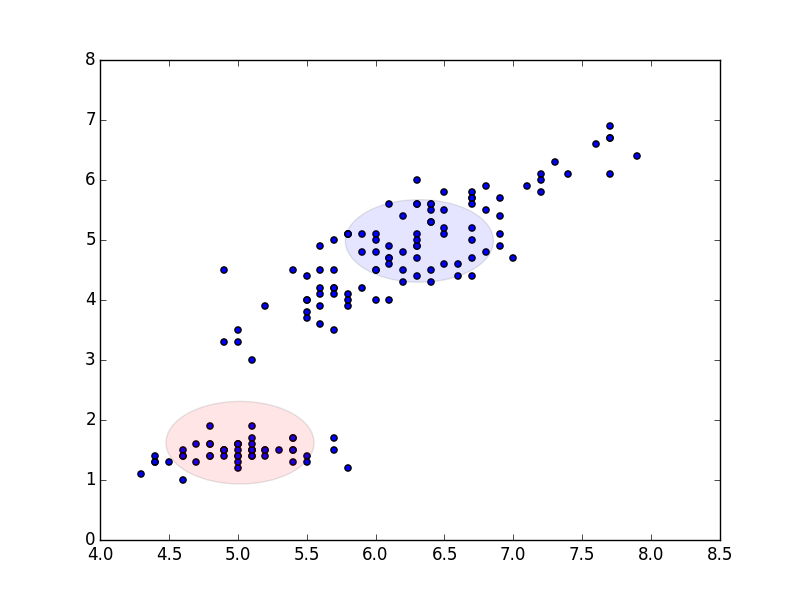
\includegraphics[scale=0.5]{../plots/irisclusters_orig.png}
  \end{center}

  The first cluster is at (6.3, 5.0) and the second is at (5.0, 1.6).  They both
  have a standard deviation of 0.54 in the x direction and 0.69 in the y direction.
  We could use these parameters to fill in the generative model:
  \begin{lstlisting}
var model = function() {
  var cluster = randomInteger(nclusters);
  return [gaussian(cluster == 0 ? 6.3 : 5.0, 0.54),
          gaussian(cluster == 0 ? 5.0 : 1.6, 0.69)];
};
  \end{lstlisting}
  This model is estimated to assign probability density $e^{-393}$ to the data, yielding a perplexity of $e^{-393/150} = 0.0728$.

  \section{Family of distributions}
  
    
  In the previous example, we that \texttt{randFunction(Categorical(2), Vector(2, Double))} represented 2 axis-aligned Gaussian clusters with equal variances.  In general, \texttt{randFunction} returns a randomized function that is a member of some generalized linear model
    determined by the desired argument types and return type.
    The distribution
    of the function's return value $y$
    is some exponential family whose natural
    parameters are determined from the arguments $x$:

    $$p_{\eta}(y | x) = \exp\left(\eta(x)^T \phi(y) - g(\eta(x))\right)$$

    Here, $\eta(x)$ is the natural parameter, $\phi(y)$ is a vector of $y$'s sufficient statistics,
    and $g$ is the log partition function.

    To determine $\eta(x)$, we label
    some subset of the sufficient statistics of both $x$ and $y$ as \emph{features}.  For the gaussian
    distribution, the sufficient statistics are $X$ and $X^2$ but the only feature is $X$.  For the
    categorical distribution \texttt{Categorical(n)}, the sufficient statistics
    and features are both $[X = 1], [X = 2], ..., [X=n - 1]$.
    The natural
    parameters corresponding to non-features are constant, while natural
    parameters corresponding to features are determined as an affine
    function of the features of the arguments.

    Let $\psi(x)$ be the features of $x$.  Then
  $$\eta(x) = \mathbf{N}^T \begin{bmatrix} 1 \\ \psi(x) \end{bmatrix}$$
    $$p_{\mathbf{N}}(y | x) = \exp\left(\begin{bmatrix} 1 \\ \psi(x) \end{bmatrix} ^T \mathbf{N} \phi(y) - g\left(\mathbf{N}^T \begin{bmatrix} 1 \\ \psi(x) \end{bmatrix}\right)\right)$$

    where $\mathbf{N}$ is a matrix containing our parameters.  It must have 0 for each entry whose row corresponds
    to a sufficient statistics of $y$ that is not a feature and whose column is not 1.
    This ensures that only the
    natural parameters that are features of $y$ are affected by $x$.  The following shows the types
    in Quipp and their corresponding sufficient statistics, features, and English descriptions.

    \begin{tabular}{| c | c | c | c|}
      \hline
      T & $\phi_T(X)$ & $\psi_T(X)$ & Random function class \\

      \hline
    \texttt{Double} & $\begin{bmatrix} X \\ X^2 \end{bmatrix}$ & $\begin{bmatrix} X \end{bmatrix}$ & Linear regression with Gaussian noise \\

      \hline
    \texttt{Categorical(n)} & $\begin{bmatrix} [X = 1] \\ [X = 2] \\ ...\\ [X = n-1] \end{bmatrix}$ & $\begin{bmatrix} [X = 1] \\ [X = 2] \\ ...\\ [X = n-1] \end{bmatrix}$ & $n$-class logistic regression \\

      \hline
    \texttt{Tuple(T1, T2)} & $\begin{bmatrix} \phi_{T1}(X_1) \\ \phi_{T2}(X_2) \end{bmatrix}$
                           & $\begin{bmatrix} \psi_{T1}(X_1) \\ \psi_{T2}(X_2) \end{bmatrix}$ &
      Independent regression of each component
      \\
      \hline
    \end{tabular}

    Note that $\texttt{Vector(n, T)}$ is shorthand for $Tuple(T, T, ..., T)$, with $n$ copies of $T$.

  \section{Example: improving the clustering model}
  Using this knowledge about the form of the random functions, we can improve the clustering model from before.
  As observed in the previous graph, the two clusters are forced to have the
  same variance. They do not fit the data well, since the data has a different
  shape in each location.  To fix this problem, we can substitute the following
  model, which uses a separate random function (and therefore a separate axis-aligned Gaussian distribution) for each cluster:
  \begin{lstlisting}
var Cluster = Categorical(2);
var Point = Vector(2, Double);
var getPointFunctions = [randFunction(Point), randFunction(Point)];

var model = function() {
  var cluster = randomValue(Cluster);
  observe(getPointFunctions[cluster]);
};
\end{lstlisting}
  Using this model, we get the following clusters:
  \begin{center}
    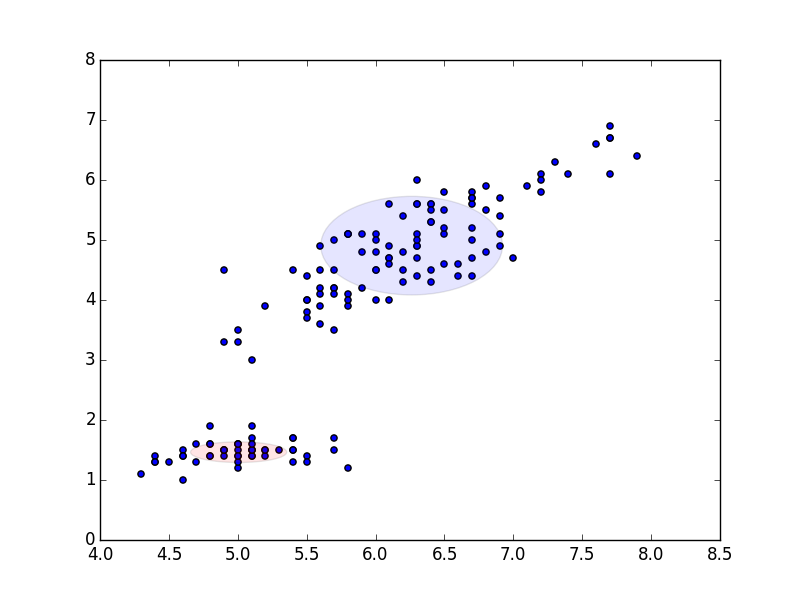
\includegraphics[scale=0.5]{../plots/irisclusters_indep.png}
  \end{center}
  This model (with the parameters filled in) is estimated to assign probability density $e^{-337}$ to the data, yielding a perplexity of 0.1058.  This is a significantly improved fit.

  The fact that the gaussian distribution for each cluster must be axis-aligned limits the degree to which the model can fit the data.   To allow each cluster to be an arbitrary Gaussian distributions (where the $x$ and $y$ coordinates may be correlated),
  we can use the following model:

\begin{lstlisting}
var Cluster = Categorical(2);
var getX = [randFunction(Double), randFunction(Double)];
var getY = [randFunction(Double, Double), randFunction(Double, Double)];

var model = function() {
  var cluster = randomInteger(nclusters);
  var x = observe(getX[cluster]);
  var y = observe(getY[cluster], x);
};
\end{lstlisting}

  Here, there are 2 random functions for each cluster, one to get the $x$ coordinate and one to get the $y$ coordinate (whose distribution may depend linearly on the $x$ coordinate).  This allows $x$ and $y$ to be correlated, improving fit:

  \begin{center}
    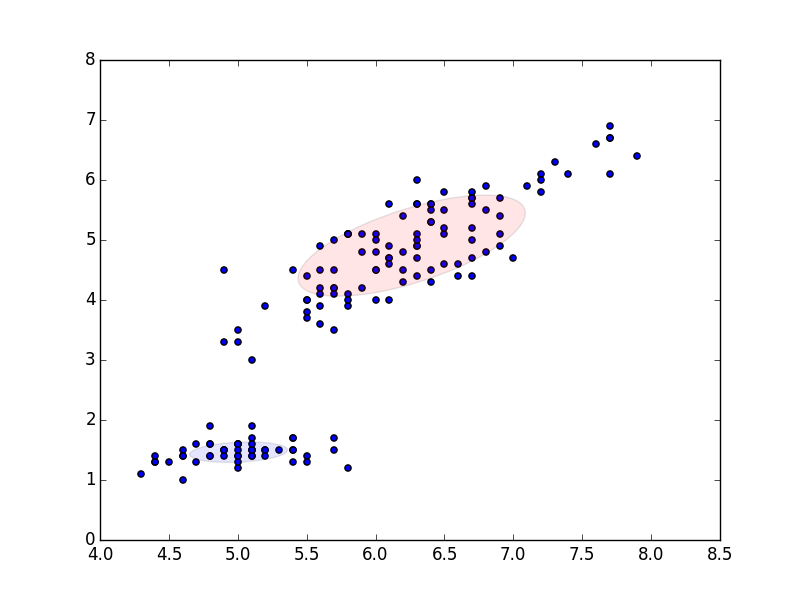
\includegraphics[scale=0.5]{../plots/irisclusters_dep.png}
  \end{center}

  This model is estimated to assign probability $e^{-269}$ to the data, yielding a perplexity of 0.166.  This is a large improvement from the previous model.



  \section{Inference}

    To infer both latent variables and parameters, we use a Monte Carlo
    expectation maximization algorithm \cite{mcem} on the probabilistic model, iterating stages of
    estimating latent variables using Metropolis Hastings and inferring
    parameters using gradient descent.

    For the expectation step, we must estimate latent variable distributions given
    fixed values for the parameters.  To do this, we can replace unknown random functions in the Quipp program
    with random functions set to use these fixed parameter values, yielding a probabilistic program.
    We use the Metropolis Hastings algorithm to perform inference in this program,
    yielding a distribution of execution traces (where each execution trace specifies the result of every
    call to a random function).  Next, for each random function, we can find all calls
    to it in the trace to get the training data.

    For the maximization step, given samples from each random function, we set the
    parameters of the function to maximize the likelihood of the samples.  To do this we,
    we use gradient descent.

    Given $(x, y)$ samples, parameter estimation to maximize log probability is a convex
    problem because the log probability function is concave as a function of $\mathbf{N}$:
    $$\log p_{\mathbf{N}}(y | x) = \begin{bmatrix} 1 \\ \psi(x) \end{bmatrix} ^T \mathbf{N} \phi(y) - g\left(\mathbf{N}^T \begin{bmatrix} 1 \\ \psi(x) \end{bmatrix}\right)$$

    This relies on the fact that $g$ is convex, but this is true in general for any exponential family distribution.
    Since the problem is convex, it is possible to use gradient descent to optimize the parameters.  Although
    the only exponential family distributions we use in this paper are the categorical and Gaussian distributions,
    we can use the same algorithms for other exponential families, such as the Poisson and gamma distributions.

  \section{Evaluation}

    To evaluate performance, for each model, we:
    \begin{itemize}
      \item
        Randomly generate parameters $\theta$
      \item
        Generate datasets $x_{train}, x_{test}$ using $\theta$
      \item
        Estimate $\log P(x_{test} | \theta)$
      \item
        Use the EM algorithm to infer approximate parameters $\hat{\theta}$ from $x_{train}$
      \item
        Estimate $\log P(x_{test} | \hat{\theta})$ and compare to $\log P(x_{test} | \theta)$
    \end{itemize}
    Estimating $\log P(x_{test} | \theta)$ is nontrivial, given that the model contains latent variables.
    We use the Sequential Monte Carlo algorithm for this.  Between observations,


  \section{Examples}

  \subsection{Clustering}
{\small
\begin{lstlisting}
var Cluster = Categorical(3);
var Point = Vector(2, Double);
var getPoint = randFunction(Cluster, Point);

var model = function() {
  var cluster = randomValue(Cluster);
  observe(getPoint, cluster);
};
\end{lstlisting}
}

In this example, we cluster 2d points into 3 different clusters.  Given a cluster, the distribution for a point is some independent Gaussian distribution.  This is similar to fuzzy c-means clustering.

\begin{center}
  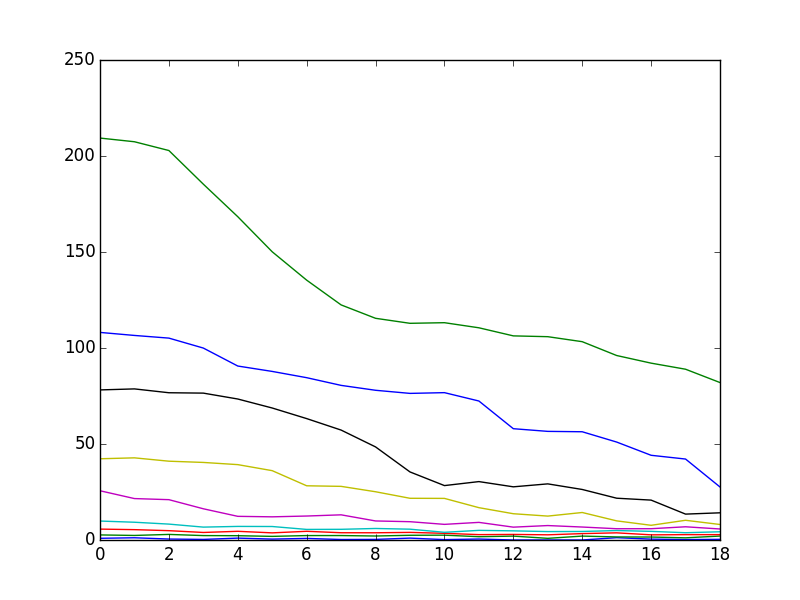
\includegraphics[scale=0.5]{../plots/accuracy_nd_clustering.png}
\end{center}

% We randomly generated parameters for this example 100 times, and each time took 100 samples and then ran 10 EM iterations.  The accuracy is defined as the maximum percentage of points assigned to the correct cluster, for any permutation of clusters.  On average, accuracy increased in each EM iteration, as shown it this graph:
% 
% \begin{center}
% 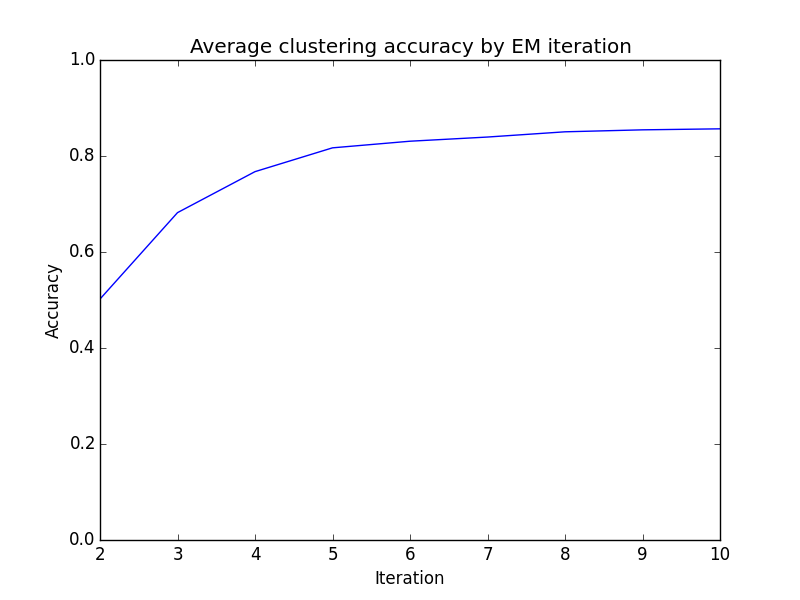
\includegraphics[scale=0.4]{cluster_accuracy.png}
% \end{center}

\subsection{Naive Bayes}

{\small
\begin{lstlisting}
var Class = Categorical(2);
var Features = Vector(10, Bool);
var classFeatures = [randFunction(Features), randFunction(Features)];

var model = function() {
  var whichClass = randomValue(Class);
  observe(classFeatures, whichClass);
};
\end{lstlisting}
}

The naive Bayes model is similar to the clustering model.  We have two classes and a feature
distribution for each.  Since each feature is boolean, we will learn
a different categorical distribution for each class.

(figure should show average classification accuracy)

  \subsection{Factor analysis}
{\small
\begin{lstlisting}
var Factors = Vector(2, Double);
var Point = Vector(5, Double);
var getPoint = randFunction(Factors, Point);

var model = function() {
  var factors = randomValue(Factors);
  return observe(getPoint, factors);
};
\end{lstlisting}
}

The factor analysis model is very similar to the clustering model.  The main difference is that we replace the categorical \texttt{ClusterType} type with a vector type.  This results in the model attempting to find each point as an affine function of a vector of standard normal values.

\begin{center}
  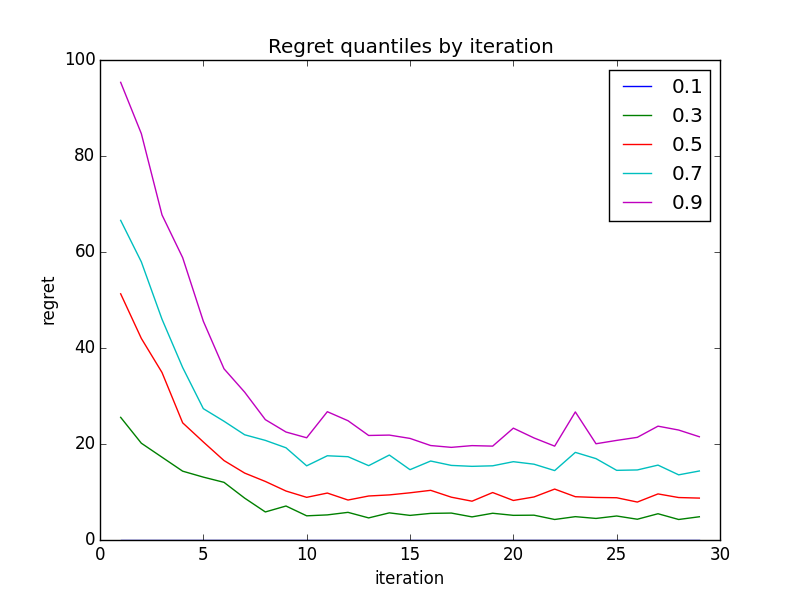
\includegraphics[scale=0.5]{../plots/accuracy_factor_analysis.png}
\end{center}

  \subsection{Hidden Markov model}
{\small
\begin{lstlisting}
var chainLength = 20;
var State = Categorical(2);
var Obs = Categorical(4);
var transFun = randFunction(State, State);
var obsFun = randFunction(State, Obs);

var observeStates = function(startState, i) {
  if (i == chainLength) {
    return [];
  } else {
    observe(obsFun, startState);
    observeStates(transFun(startState), i+1);
  }
};

var model = function() {
  return observeStates(randomValue(State), 0);
};
\end{lstlisting}
}

In this example, we use the unknown function \texttt{transFun} for state transitions and \texttt{obsFun} for observations.  This means that we will learn both the state transitions and the observation distribution.

\begin{center}
  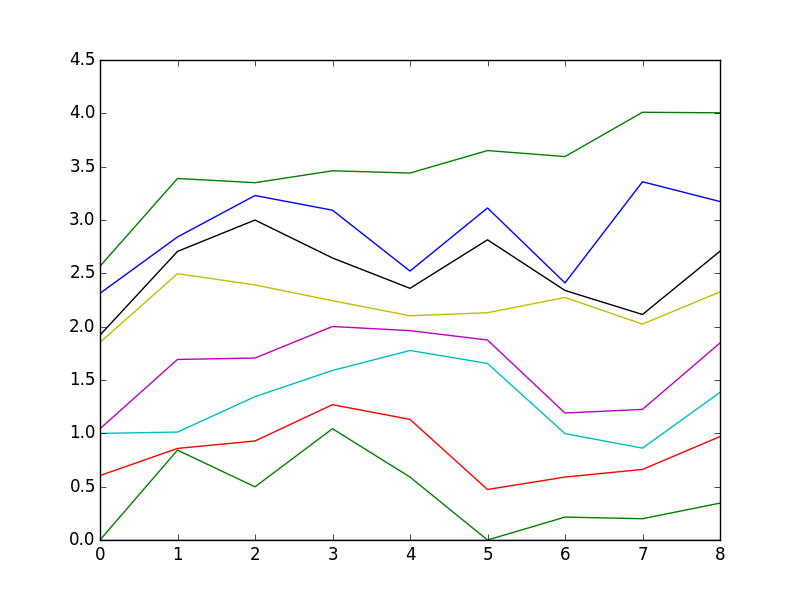
\includegraphics[scale=0.5]{../plots/accuracy_hmm.png}
\end{center}

\subsection{Latent Dirichlet allocation}
{\small
\begin{lstlisting}
var maxWordsPerDocument = 100;
var Class = Categorical(3);
var Word = Categorical(10);
var classToWord = randFunction(Class, Word);

var model = function() {
  var whichClass = randomValue(Class);
  var nWords = observe('len' + docIndex, randomIntegerERP, maxWordsPerDocument);
  repeat(nWords, function(wordIndex) {
    observe(classToWord, whichClass);
  });
};
\end{lstlisting}
}

In this example, we use the unknown function \texttt{classToWord} to map classes to word distributions.  Note that each column of the matrix of parameters for \texttt{classToWord} will represent a categorical distribution over words, and there will be one column for each class.

\begin{center}
  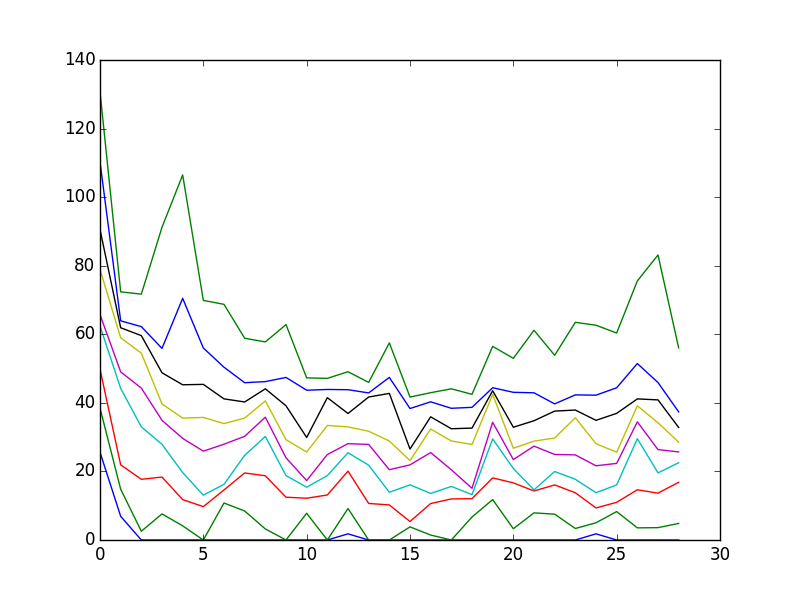
\includegraphics[scale=0.5]{../plots/accuracy_lda.png}
\end{center}
\subsection{Neural network}

{\small
\begin{lstlisting}
var Input = Vector(30, Bool);
var Hidden = Vector(10, Bool);
var Output = Bool;

var inputToHidden = randFunction(Input, Hidden);
var hiddenToOutput = randFunction(Hidden, Output);

var model = function() {
  var inputLayer = randomValue(Input);
  var hiddenLayer = inputToHidden(inputs[sampIndex]);
  observe(hiddenToOutput, hiddenLayer);
};
\end{lstlisting}
}

  \section{Discussion}

  We have found that it is possible to write many useful machine learning models as Quipp programs and then use generic algorithms for inference.  Furthermore, performance is <???>.  This should make it much easier for non-experts to write useful machine learning models.
  
  In the future, it will be useful to expand the set of types supported.  It is possible to define reasonable default distributions for non-recursive algebraic data types, and it may also be possible to define them for recursive algebraic data types using catamorphisms.  Also, it will be useful to create a more usable interface to infer parameters and perform additional data pracessing given these parameters.

\bibliography{bibliography}{}
\bibliographystyle{plain}


\end{document}

